% pdflatex ten-graphing-problems.tex && del ten-graphing-problems.aux, ten-graphing-problems.out, ten-graphing-problems.log && start ten-graphing-problems.pdf
% cd ..\..\Users\NikitaSkybytskyi\Desktop\c3s1\complex-analysis
\documentclass[a4paper, 12pt]{article}
\usepackage[utf8]{inputenc}
\usepackage[english, ukrainian]{babel}

\usepackage{amsmath, amssymb}
\usepackage{multicol}
\usepackage{graphicx}
\usepackage{float}
\usepackage{multicol}

\usepackage{amsthm}
\newtheorem{theorem}{Теорема}[subsection]
\newtheorem*{theorem*}{Теорема}
\newtheorem{lemma}{Лема}[subsection]
\newtheorem*{lemma*}{Лема}
\newtheorem*{remark*}{Зауваження}
\theoremstyle{definition}
\newtheorem*{definition}{Визначення}
\newtheorem{problem}{Задача}[section]
\newtheorem*{solution}{Розв'язок}
\newtheorem{example}{Приклад}
\newtheorem*{example*}{Приклад}
\newtheorem*{hint}{Вказівка}

\newcommand{\Max}{\displaystyle\max\limits}
\newcommand{\Sum}{\displaystyle\sum\limits}
\newcommand{\Int}{\displaystyle\int\limits}
\newcommand{\Lim}{\displaystyle\lim\limits}

\newcommand{\RR}{\mathbb{R}}
\newcommand{\ZZ}{\mathbb{Z}}

\newcommand*\diff{\mathop{}\!\mathrm{d}}
\newcommand*\Diff[1]{\mathop{}\!\mathrm{d^#1}}

\DeclareMathOperator{\Real}{Re}
\DeclareMathOperator{\Imag}{Im}

\DeclareMathOperator{\Arg}{Arg}

\DeclareMathOperator{\Ln}{Ln}

\DeclareMathOperator{\Arctan}{Arctan}
\DeclareMathOperator{\Arcsin}{Arcsin}
\DeclareMathOperator{\Arccos}{Arccos}
\DeclareMathOperator{\Arccosh}{Arccosh}
\DeclareMathOperator{\Arctanh}{Arctanh}

\DeclareMathOperator{\arcsinh}{arcsinh}
\DeclareMathOperator{\arccosh}{arccosh}
\DeclareMathOperator{\arctanh}{arctanh}
\DeclareMathOperator{\arccoth}{arccoth}

\newcommand{\varLimsup}{\varlimsup\limits}

\makeatletter
\newcommand\xLeftrightarrow[2][]{%
  \ext@arrow 9999{\longLeftrightarrowfill@}{#1}{#2}}
\newcommand\longLeftrightarrowfill@{%
  \arrowfill@\Leftarrow\relbar\Rightarrow}
\makeatother

\renewcommand{\epsilon}{\varepsilon}
\renewcommand{\phi}{\varphi}

\allowdisplaybreaks
\setlength\parindent{0pt}
\numberwithin{equation}{subsection}

\usepackage{xcolor}
\usepackage{hyperref}
\hypersetup{unicode=true,colorlinks=true,linktoc=all,linkcolor=red}

\numberwithin{equation}{section}% reset equation counter for sections
\numberwithin{equation}{subsection}
% Omit `.0` in equation numbers for non-existent subsections.
\renewcommand*{\theequation}{%
  \ifnum\value{subsection}=0 %
    \thesection
  \else
    \thesubsection
  \fi
  .\arabic{equation}%
}


\numberwithin{equation}{section}

\begin{document}

\setcounter{section}{1}

\setcounter{problem}{22}

У задачах 1.23--1.34 необхідно з'ясувати геометричний зміст вказаних співвідношень.
\begin{problem}
	$|z - z_0| < R$; $|z - z_0| > R$; $|z - z_0| = R$.
\end{problem}
\begin{solution}
	Внутрішність круга з центром $z_0$ і радіусом $R$, зовнішність цього круга, і коло яке є межею цього круга:
	\begin{figure}[H]
		\centering
		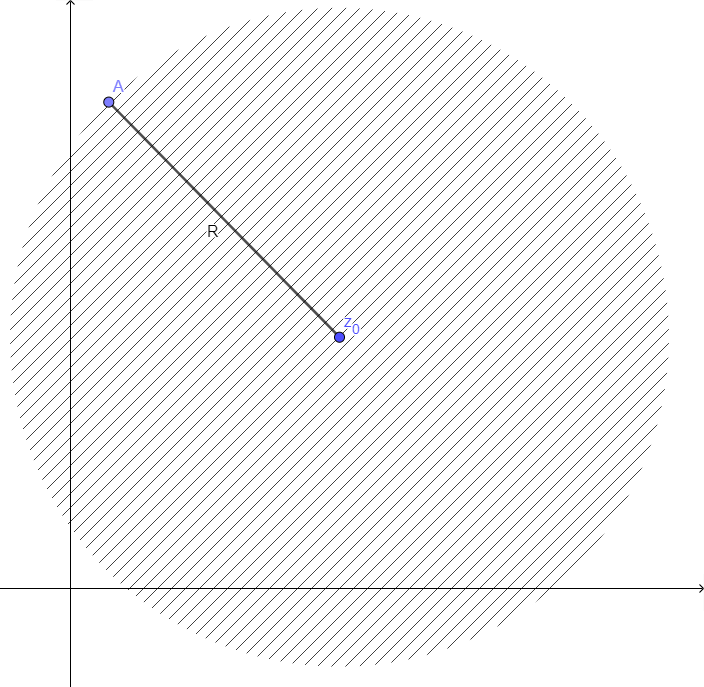
\includegraphics[width=.3\linewidth]{fig-4.png}
		\quad
		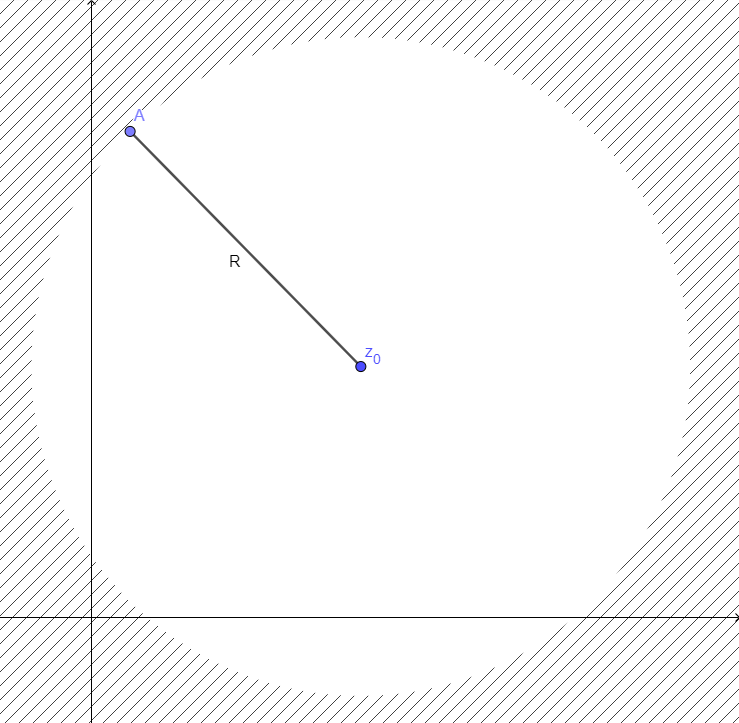
\includegraphics[width=.3\linewidth]{fig-5.png}
		\quad
		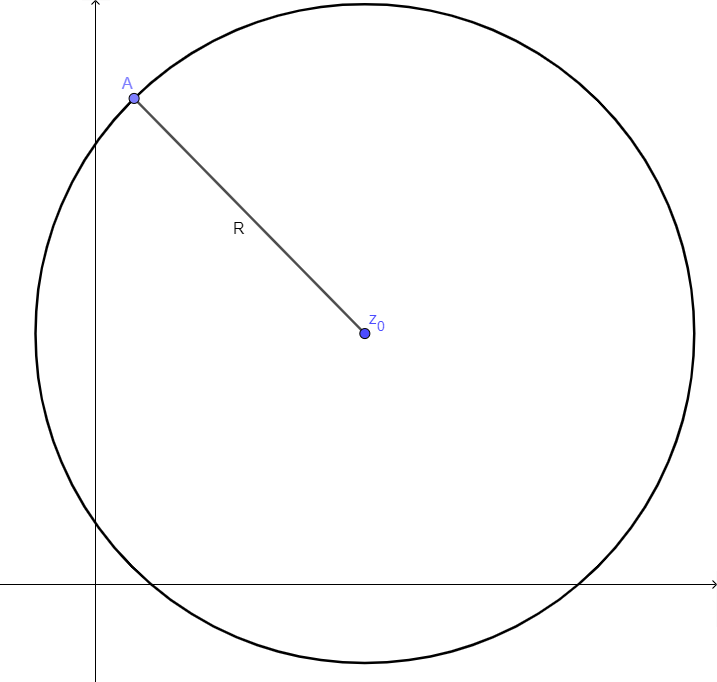
\includegraphics[width=.3\linewidth]{fig-6.png}
	\end{figure}
\end{solution}
	
\begin{problem}
	$|z - 2| + |z + 2| = 5$.
\end{problem}
\begin{solution}
	Еліпс з фокусами $-2$, $2$ і ``радіусом'' 5:
	\begin{figure}[H]
		\centering
		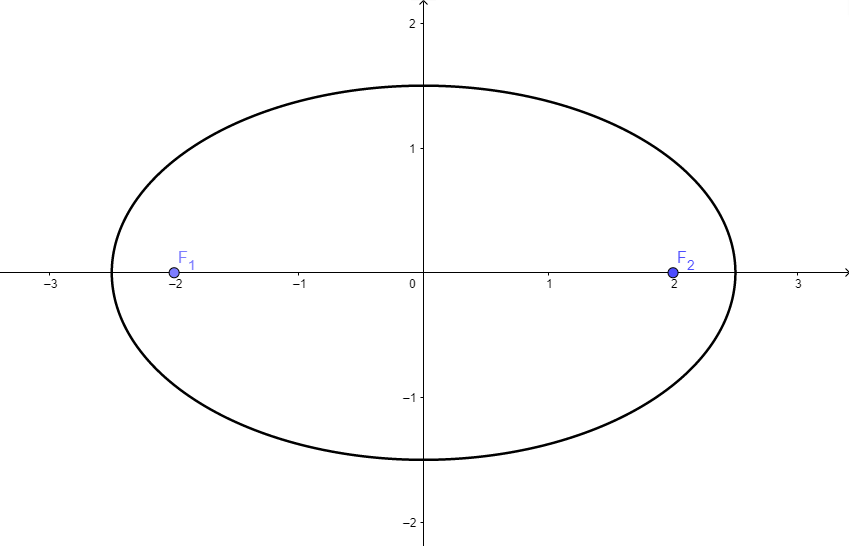
\includegraphics[width=\linewidth]{fig-7.png}
	\end{figure}
\end{solution}

\begin{problem}
	$|z-2| - |z+2| > 3$.
\end{problem}
\begin{solution}
	Внутрішність ``лівої'' гілки гіперболи з фокусами $-2$, $2$ і ``радіусом'' 3:
	\begin{figure}[H]
		\centering
		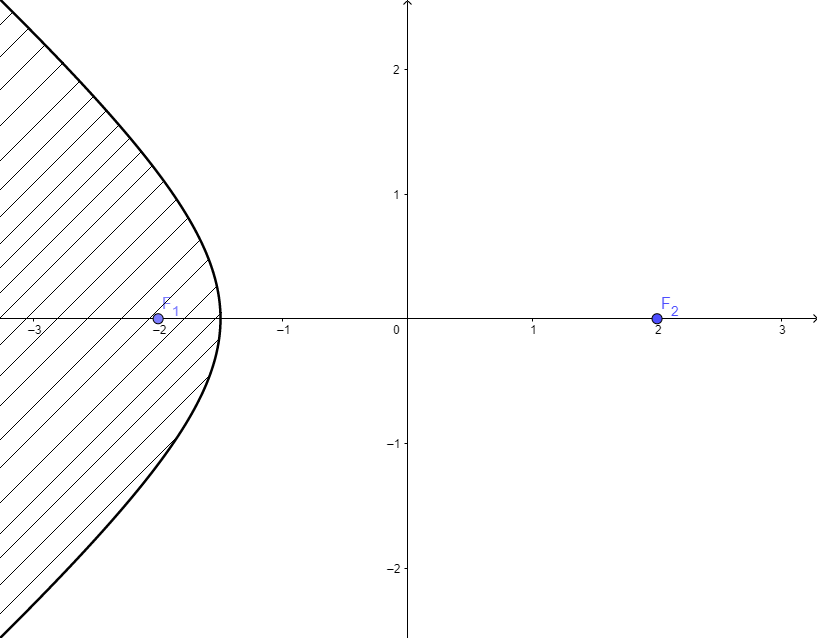
\includegraphics[width=.85\linewidth]{fig-8.png}
	\end{figure}
\end{solution}

\begin{problem}
	$|z - z_1| = |z - z_2|$.
\end{problem}
\begin{solution}
	Серединний перпендикуляр до відрізку, що сполучає точки $z_1$ і $z_2$:
	\begin{figure}[H]
		\centering
		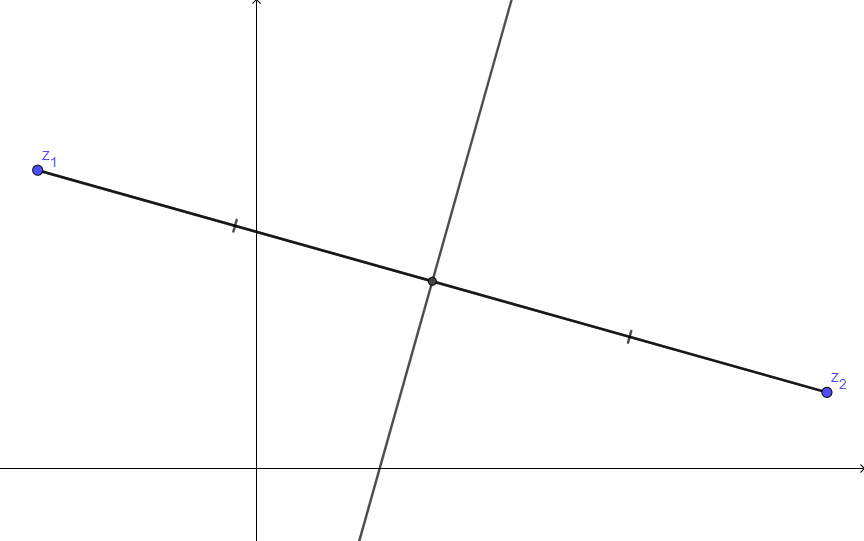
\includegraphics[width=.85\linewidth]{fig-9.png}
	\end{figure}
\end{solution}

\begin{problem}
	$\Real z \ge C$; $\Imag z < C$.
\end{problem}
\begin{solution}
	``Права'' (замкнена, тобто із прямою, що є границею) півплощина відносно прямої $x = C$. \\

	``Нижня'' (відкрита, тобто без прямої, що є границею) півплощина відсносно прямої $y = C$.
\end{solution}

\begin{problem}
	$0 < \Real (iz) < 1$.
\end{problem}
\begin{solution}
	$\Real (iz) = \Real (i(x + iy)) = -y$, тому вказаний об'єкт -- (відкрита) горизонтальна смуга $-1 < y < 0$.
\end{solution}

\begin{problem}
	$\alpha < \arg z < \beta$; $\alpha < \arg (z - z_0) < \beta$ ($-\pi < \alpha < \beta \le \pi$).
\end{problem}
\begin{solution}
	(Відкритий) кут від $\alpha$ до $\beta$ з центром в $0$ та $z_0$ відповідно.
\end{solution}

\begin{problem}
	$|z| = \Real z + 1$.
\end{problem}
\begin{solution} % thanks to Olexander Prikhodko
	Парабола з фокусом 0 і директрисою $x = -1$.
\end{solution}

\begin{problem}
	$\Real z + \Imag z < 1$.
\end{problem}
\begin{solution} % thanks to Vladyslav Verteletskyi
	``Ліва нижня'' півплощина відносно прямої $x + y = 1$.
\end{solution}

\begin{problem}
	$\Imag \frac{z-z_1}{z-z_2}=0$; $\Real \frac{z-z_1}{z-z_2}=0$;
\end{problem}
\begin{solution} % thanks to Olexander Prikhodko
	$\Imag \frac{z-z_1}{z-z_2}=0 \iff \arg (z - z_1) = \arg (z - z_2)$, тобто $z$ належить прямій, що сполучає точки $z_1$ та $z_2$. \\

	$\Real \frac{z-z_1}{z-z_2}=0 \iff \arg(z-z_1)=\pi/2+\arg(z-z_2)$, тобто відрізки, що сполучають точки $z$ і $z_1$ та $z$ і $z_2$ перпендикулярні, тобто $z$ належить колу, побудованому на відрізку, що сполучає точки $z_1$ і $z_2$, як на діаметрі. 
\end{solution}

\begin{problem}
	$|2z| > |1+z^2|$.
\end{problem}
\begin{solution}
	\[|2z| > |1+z^2| \iff \left(|z - i| - \sqrt{2}\right) \cdot \left(|z + i| - \sqrt{2}\right) < 0,\] тому вказана множина є $\mathcal{K}_{\sqrt{2}}(-i) \Delta \mathcal{K}_{\sqrt{2}}(i)$.
\end{solution}

\end{document}